\documentclass[14pt]{diploma}

\usepackage[T2A]{fontenc}
\usepackage{pscyr}
\usepackage[cp1251]{inputenc}

\usepackage{lscape}

\pagestyle{empty}

\newcounter{slide}

\newcommand{\slide}{
    \stepcounter{slide}
    \fbox{\includegraphics[page=\theslide,width=0.65\textwidth]{../Slides/Bezborodov_Presentation_Parallel_implementation_of_the_ellipsoids_method_for_optimization_problems_of_large_dimension.pdf}}
}

\newcommand{\page}{
    \begin{table}[h!]
        \centering
        \begin{tabular}{cc}
        \slide & \slide
        \end{tabular}
    \end{table}
    \begin{table}[h!]
        \centering
        \begin{tabular}{p{0.8\textwidth}}
        \\
        \\ \hline
        \\
        \\ \hline
        \\
        \\ \hline
        \\
        \\ \hline
        \end{tabular}
    \end{table}
    \newpage
}

\begin{document}

\begin{enumerate}

\item The title of my Master's dissertation is <<Parallel implementation of the ellipsoids method for optimization problems of large dimension>>

\item Today we are going to talk about the ellipsoids method -- a key discussion thread of the dissertation, about matrices and it's processing and finally about applied implementation of the method

\item Now we can define the purposes or goals of that work. We'd like to develop parallel implementation of the ellipsoids method that support arbitrary precision arithmetic and demonstrate how to use developed software for solving optimization problems of large dimension

\item Respectively, first thing we need to develop a program implementation is to examine computational complexity of the existing algorithm. Then we can analyse each step of the method to figure out the most time-consuming operations (as you probably know the most matrix operations is time-consuming) to parallel it and speed up or accelerate whole algorithm, or we can say, to reduce algorithm run time

\item Before we start, let's shortly browse the history of the ellipsoids method algorithm

\item The method was independently proposed in three different periods of time by different scientists. Note that all of them are soviet mathematicians

\item Next is the geometry briefing

\item It's pretty hard to explain the details of how the method works, but the main idea is simple. If to stretch the space with certain factor in the particular direction, the ellipsoid becomes a ball in the new space

\item Let me show where the ellipsoids method can be applied

\item Here a list of the applied convex programming problems that can be solved by the method

\item The algorithm of the method

\item All the algorithm steps are listed on the slide. The idea is to construct the ellipsoid of as small as possible volume to locate optimal point

\item This theorem guarantee that the algorithm finds out optimal point if all of the preconditions are hold

\item As I already mentioned most of the matrix operations are very time-consuming. So, there are several possibilities to speed up the performance

\item In parallel computing, the fork�join model is a way of setting up and executing parallel programs, such that execution branches off in parallel at designated points in the program, to "join" (merge) at a subsequent point and resume sequential execution. Parallel sections may fork recursively until a certain task granularity is reached

\item Here are the ways how we can split a matrix and distribute it between threads

\item By using such a way of executing a program we can expect some rate of acceleration

\item So, here the acceleration rate we reached in practice for matrix addition

\item For multiplication

\item And for time reducing

\item Now let's talk about some computer experiments

\item For the first sample we have a objective function and two restrictions. At the left bottom corner you can see the accurate optimum and at the right -- the optimum calculated with the ellipsoids method algorithm

\item Now you can see an optimization problem of large dimension which has been solved by using different number of threads

\item At in conclusion we'd like to say that ellipsoids method allows to solve a wide range of optimization problems 
in various fields of human activities

\item Thank you

\end{enumerate}

\end{document}